\documentclass[]{article}
\usepackage{lmodern}
\usepackage{amssymb,amsmath}
\usepackage{ifxetex,ifluatex}
\usepackage{fixltx2e} % provides \textsubscript
\ifnum 0\ifxetex 1\fi\ifluatex 1\fi=0 % if pdftex
  \usepackage[T1]{fontenc}
  \usepackage[utf8]{inputenc}
\else % if luatex or xelatex
  \ifxetex
    \usepackage{mathspec}
  \else
    \usepackage{fontspec}
  \fi
  \defaultfontfeatures{Ligatures=TeX,Scale=MatchLowercase}
\fi
% use upquote if available, for straight quotes in verbatim environments
\IfFileExists{upquote.sty}{\usepackage{upquote}}{}
% use microtype if available
\IfFileExists{microtype.sty}{%
\usepackage{microtype}
\UseMicrotypeSet[protrusion]{basicmath} % disable protrusion for tt fonts
}{}
\usepackage[margin=1in]{geometry}
\usepackage{hyperref}
\hypersetup{unicode=true,
            pdftitle={TD1},
            pdfborder={0 0 0},
            breaklinks=true}
\urlstyle{same}  % don't use monospace font for urls
\usepackage{color}
\usepackage{fancyvrb}
\newcommand{\VerbBar}{|}
\newcommand{\VERB}{\Verb[commandchars=\\\{\}]}
\DefineVerbatimEnvironment{Highlighting}{Verbatim}{commandchars=\\\{\}}
% Add ',fontsize=\small' for more characters per line
\usepackage{framed}
\definecolor{shadecolor}{RGB}{248,248,248}
\newenvironment{Shaded}{\begin{snugshade}}{\end{snugshade}}
\newcommand{\KeywordTok}[1]{\textcolor[rgb]{0.13,0.29,0.53}{\textbf{#1}}}
\newcommand{\DataTypeTok}[1]{\textcolor[rgb]{0.13,0.29,0.53}{#1}}
\newcommand{\DecValTok}[1]{\textcolor[rgb]{0.00,0.00,0.81}{#1}}
\newcommand{\BaseNTok}[1]{\textcolor[rgb]{0.00,0.00,0.81}{#1}}
\newcommand{\FloatTok}[1]{\textcolor[rgb]{0.00,0.00,0.81}{#1}}
\newcommand{\ConstantTok}[1]{\textcolor[rgb]{0.00,0.00,0.00}{#1}}
\newcommand{\CharTok}[1]{\textcolor[rgb]{0.31,0.60,0.02}{#1}}
\newcommand{\SpecialCharTok}[1]{\textcolor[rgb]{0.00,0.00,0.00}{#1}}
\newcommand{\StringTok}[1]{\textcolor[rgb]{0.31,0.60,0.02}{#1}}
\newcommand{\VerbatimStringTok}[1]{\textcolor[rgb]{0.31,0.60,0.02}{#1}}
\newcommand{\SpecialStringTok}[1]{\textcolor[rgb]{0.31,0.60,0.02}{#1}}
\newcommand{\ImportTok}[1]{#1}
\newcommand{\CommentTok}[1]{\textcolor[rgb]{0.56,0.35,0.01}{\textit{#1}}}
\newcommand{\DocumentationTok}[1]{\textcolor[rgb]{0.56,0.35,0.01}{\textbf{\textit{#1}}}}
\newcommand{\AnnotationTok}[1]{\textcolor[rgb]{0.56,0.35,0.01}{\textbf{\textit{#1}}}}
\newcommand{\CommentVarTok}[1]{\textcolor[rgb]{0.56,0.35,0.01}{\textbf{\textit{#1}}}}
\newcommand{\OtherTok}[1]{\textcolor[rgb]{0.56,0.35,0.01}{#1}}
\newcommand{\FunctionTok}[1]{\textcolor[rgb]{0.00,0.00,0.00}{#1}}
\newcommand{\VariableTok}[1]{\textcolor[rgb]{0.00,0.00,0.00}{#1}}
\newcommand{\ControlFlowTok}[1]{\textcolor[rgb]{0.13,0.29,0.53}{\textbf{#1}}}
\newcommand{\OperatorTok}[1]{\textcolor[rgb]{0.81,0.36,0.00}{\textbf{#1}}}
\newcommand{\BuiltInTok}[1]{#1}
\newcommand{\ExtensionTok}[1]{#1}
\newcommand{\PreprocessorTok}[1]{\textcolor[rgb]{0.56,0.35,0.01}{\textit{#1}}}
\newcommand{\AttributeTok}[1]{\textcolor[rgb]{0.77,0.63,0.00}{#1}}
\newcommand{\RegionMarkerTok}[1]{#1}
\newcommand{\InformationTok}[1]{\textcolor[rgb]{0.56,0.35,0.01}{\textbf{\textit{#1}}}}
\newcommand{\WarningTok}[1]{\textcolor[rgb]{0.56,0.35,0.01}{\textbf{\textit{#1}}}}
\newcommand{\AlertTok}[1]{\textcolor[rgb]{0.94,0.16,0.16}{#1}}
\newcommand{\ErrorTok}[1]{\textcolor[rgb]{0.64,0.00,0.00}{\textbf{#1}}}
\newcommand{\NormalTok}[1]{#1}
\usepackage{graphicx,grffile}
\makeatletter
\def\maxwidth{\ifdim\Gin@nat@width>\linewidth\linewidth\else\Gin@nat@width\fi}
\def\maxheight{\ifdim\Gin@nat@height>\textheight\textheight\else\Gin@nat@height\fi}
\makeatother
% Scale images if necessary, so that they will not overflow the page
% margins by default, and it is still possible to overwrite the defaults
% using explicit options in \includegraphics[width, height, ...]{}
\setkeys{Gin}{width=\maxwidth,height=\maxheight,keepaspectratio}
\IfFileExists{parskip.sty}{%
\usepackage{parskip}
}{% else
\setlength{\parindent}{0pt}
\setlength{\parskip}{6pt plus 2pt minus 1pt}
}
\setlength{\emergencystretch}{3em}  % prevent overfull lines
\providecommand{\tightlist}{%
  \setlength{\itemsep}{0pt}\setlength{\parskip}{0pt}}
\setcounter{secnumdepth}{0}
% Redefines (sub)paragraphs to behave more like sections
\ifx\paragraph\undefined\else
\let\oldparagraph\paragraph
\renewcommand{\paragraph}[1]{\oldparagraph{#1}\mbox{}}
\fi
\ifx\subparagraph\undefined\else
\let\oldsubparagraph\subparagraph
\renewcommand{\subparagraph}[1]{\oldsubparagraph{#1}\mbox{}}
\fi

%%% Use protect on footnotes to avoid problems with footnotes in titles
\let\rmarkdownfootnote\footnote%
\def\footnote{\protect\rmarkdownfootnote}

%%% Change title format to be more compact
\usepackage{titling}

% Create subtitle command for use in maketitle
\newcommand{\subtitle}[1]{
  \posttitle{
    \begin{center}\large#1\end{center}
    }
}

\setlength{\droptitle}{-2em}

  \title{TD1}
    \pretitle{\vspace{\droptitle}\centering\huge}
  \posttitle{\par}
    \author{}
    \preauthor{}\postauthor{}
    \date{}
    \predate{}\postdate{}
  

\begin{document}
\maketitle

{
\setcounter{tocdepth}{2}
\tableofcontents
}
\subsection{Exercice 1}\label{exercice-1}

\begin{enumerate}
\def\labelenumi{\arabic{enumi}.}
\tightlist
\item
  Create a vector of number

  \begin{itemize}
  \tightlist
  \item
    The list from 1 to 100
  \end{itemize}

\begin{Shaded}
\begin{Highlighting}[]
\KeywordTok{seq}\NormalTok{(}\DecValTok{1}\NormalTok{,}\DecValTok{100}\NormalTok{)}
\end{Highlighting}
\end{Shaded}

\begin{verbatim}
##   [1]   1   2   3   4   5   6   7   8   9  10  11  12  13  14  15  16  17
##  [18]  18  19  20  21  22  23  24  25  26  27  28  29  30  31  32  33  34
##  [35]  35  36  37  38  39  40  41  42  43  44  45  46  47  48  49  50  51
##  [52]  52  53  54  55  56  57  58  59  60  61  62  63  64  65  66  67  68
##  [69]  69  70  71  72  73  74  75  76  77  78  79  80  81  82  83  84  85
##  [86]  86  87  88  89  90  91  92  93  94  95  96  97  98  99 100
\end{verbatim}

  \begin{itemize}
  \tightlist
  \item
    A number list/sequence for 10, 20, 25, 50, repeated 5 times ( 10 20
    25 50 10 20 25 50 10 20 25 50 10 20 25 50 10 20 25 50)
  \end{itemize}

\begin{Shaded}
\begin{Highlighting}[]
\KeywordTok{rep}\NormalTok{(}\KeywordTok{c}\NormalTok{(}\DecValTok{10}\NormalTok{,}\DecValTok{20}\NormalTok{,}\DecValTok{25}\NormalTok{,}\DecValTok{50}\NormalTok{),}\DecValTok{5}\NormalTok{)}
\end{Highlighting}
\end{Shaded}

\begin{verbatim}
##  [1] 10 20 25 50 10 20 25 50 10 20 25 50 10 20 25 50 10 20 25 50
\end{verbatim}

  \begin{itemize}
  \tightlist
  \item
    a list from 1 to 100, with a step of 5
  \end{itemize}

\begin{Shaded}
\begin{Highlighting}[]
\KeywordTok{seq}\NormalTok{(}\DecValTok{1}\NormalTok{,}\DecValTok{100}\NormalTok{,}\DecValTok{5}\NormalTok{)}
\end{Highlighting}
\end{Shaded}

\begin{verbatim}
##  [1]  1  6 11 16 21 26 31 36 41 46 51 56 61 66 71 76 81 86 91 96
\end{verbatim}

  \begin{itemize}
  \tightlist
  \item
    Repeat 10 times the number 12
  \end{itemize}

\begin{Shaded}
\begin{Highlighting}[]
\KeywordTok{rep}\NormalTok{(}\DecValTok{12}\NormalTok{,}\DecValTok{10}\NormalTok{)}
\end{Highlighting}
\end{Shaded}

\begin{verbatim}
##  [1] 12 12 12 12 12 12 12 12 12 12
\end{verbatim}
\item
  A vector with the number 1, 2, 3 with a repetition of each 4 times
  with in addition a repetition of the sequence of 4 times

  \begin{itemize}
  \tightlist
  \item
    Put this vector in the object « VEC »
  \end{itemize}

\begin{Shaded}
\begin{Highlighting}[]
\NormalTok{VEC =}\StringTok{ }\KeywordTok{rep}\NormalTok{(}\KeywordTok{c}\NormalTok{(}\DecValTok{1}\NormalTok{,}\DecValTok{2}\NormalTok{,}\DecValTok{3}\NormalTok{),}\DataTypeTok{each =} \DecValTok{4}\NormalTok{, }\DataTypeTok{times =} \DecValTok{4}\NormalTok{)}
\NormalTok{VEC}
\end{Highlighting}
\end{Shaded}

\begin{verbatim}
##  [1] 1 1 1 1 2 2 2 2 3 3 3 3 1 1 1 1 2 2 2 2 3 3 3 3 1 1 1 1 2 2 2 2 3 3 3
## [36] 3 1 1 1 1 2 2 2 2 3 3 3 3
\end{verbatim}

  \begin{itemize}
  \tightlist
  \item
    Multiply all the element of VEC by 5
  \end{itemize}

\begin{Shaded}
\begin{Highlighting}[]
\NormalTok{VEC =}\StringTok{ }\NormalTok{VEC }\OperatorTok{*}\StringTok{ }\DecValTok{5}
\NormalTok{VEC}
\end{Highlighting}
\end{Shaded}

\begin{verbatim}
##  [1]  5  5  5  5 10 10 10 10 15 15 15 15  5  5  5  5 10 10 10 10 15 15 15
## [24] 15  5  5  5  5 10 10 10 10 15 15 15 15  5  5  5  5 10 10 10 10 15 15
## [47] 15 15
\end{verbatim}

  \begin{itemize}
  \tightlist
  \item
    Calculate the median and the quantile of 75\%
  \end{itemize}

\begin{Shaded}
\begin{Highlighting}[]
\KeywordTok{quantile}\NormalTok{(VEC, }\FloatTok{0.5}\NormalTok{) }\CommentTok{# Median}
\end{Highlighting}
\end{Shaded}

\begin{verbatim}
## 50% 
##  10
\end{verbatim}

\begin{Shaded}
\begin{Highlighting}[]
\KeywordTok{quantile}\NormalTok{(VEC, }\FloatTok{0.75}\NormalTok{)}
\end{Highlighting}
\end{Shaded}

\begin{verbatim}
## 75% 
##  15
\end{verbatim}
\item
  Create a vector with a serie of number from 1 to 2000 with a step of
  10

  \begin{itemize}
  \tightlist
  \item
    Put it in the object « vec »
  \end{itemize}

\begin{Shaded}
\begin{Highlighting}[]
\NormalTok{vec =}\StringTok{ }\KeywordTok{seq}\NormalTok{(}\DecValTok{1}\NormalTok{,}\DecValTok{2000}\NormalTok{,}\DecValTok{10}\NormalTok{)}
\NormalTok{vec}
\end{Highlighting}
\end{Shaded}

\begin{verbatim}
##   [1]    1   11   21   31   41   51   61   71   81   91  101  111  121  131
##  [15]  141  151  161  171  181  191  201  211  221  231  241  251  261  271
##  [29]  281  291  301  311  321  331  341  351  361  371  381  391  401  411
##  [43]  421  431  441  451  461  471  481  491  501  511  521  531  541  551
##  [57]  561  571  581  591  601  611  621  631  641  651  661  671  681  691
##  [71]  701  711  721  731  741  751  761  771  781  791  801  811  821  831
##  [85]  841  851  861  871  881  891  901  911  921  931  941  951  961  971
##  [99]  981  991 1001 1011 1021 1031 1041 1051 1061 1071 1081 1091 1101 1111
## [113] 1121 1131 1141 1151 1161 1171 1181 1191 1201 1211 1221 1231 1241 1251
## [127] 1261 1271 1281 1291 1301 1311 1321 1331 1341 1351 1361 1371 1381 1391
## [141] 1401 1411 1421 1431 1441 1451 1461 1471 1481 1491 1501 1511 1521 1531
## [155] 1541 1551 1561 1571 1581 1591 1601 1611 1621 1631 1641 1651 1661 1671
## [169] 1681 1691 1701 1711 1721 1731 1741 1751 1761 1771 1781 1791 1801 1811
## [183] 1821 1831 1841 1851 1861 1871 1881 1891 1901 1911 1921 1931 1941 1951
## [197] 1961 1971 1981 1991
\end{verbatim}

  \begin{itemize}
  \tightlist
  \item
    Extract the 10 th value of vec
  \end{itemize}

\begin{Shaded}
\begin{Highlighting}[]
\NormalTok{vec[}\DecValTok{10}\NormalTok{]}
\end{Highlighting}
\end{Shaded}

\begin{verbatim}
## [1] 91
\end{verbatim}

  \begin{itemize}
  \tightlist
  \item
    Display a sub-vector called « vec2 » that corresponds to the values
    from 2 to 6
  \end{itemize}

\begin{Shaded}
\begin{Highlighting}[]
\NormalTok{vec2 =}\StringTok{ }\NormalTok{vec[}\DecValTok{2}\OperatorTok{:}\DecValTok{6}\NormalTok{]}
\NormalTok{vec2}
\end{Highlighting}
\end{Shaded}

\begin{verbatim}
## [1] 11 21 31 41 51
\end{verbatim}

  \begin{itemize}
  \tightlist
  \item
    Replace the last value of vec2 by 100
  \end{itemize}

\begin{Shaded}
\begin{Highlighting}[]
\NormalTok{vec2[}\KeywordTok{length}\NormalTok{(vec2)] =}\StringTok{ }\DecValTok{100}
\NormalTok{vec2}
\end{Highlighting}
\end{Shaded}

\begin{verbatim}
## [1]  11  21  31  41 100
\end{verbatim}

  \begin{itemize}
  \tightlist
  \item
    Display vec2 without its 3th value and store it in vec3
  \end{itemize}

\begin{Shaded}
\begin{Highlighting}[]
\NormalTok{vec3 =}\StringTok{ }\NormalTok{vec2[}\OperatorTok{-}\DecValTok{3}\NormalTok{]}
\NormalTok{vec3}
\end{Highlighting}
\end{Shaded}

\begin{verbatim}
## [1]  11  21  41 100
\end{verbatim}

  \begin{itemize}
  \tightlist
  \item
    Replace all the values \textgreater{}= 30 by 30
  \end{itemize}

\begin{Shaded}
\begin{Highlighting}[]
\NormalTok{vec3[vec3 }\OperatorTok{>=}\StringTok{ }\DecValTok{30}\NormalTok{] =}\StringTok{ }\DecValTok{30}
\NormalTok{vec3}
\end{Highlighting}
\end{Shaded}

\begin{verbatim}
## [1] 11 21 30 30
\end{verbatim}
\end{enumerate}

\subsection{Exercice 2 : Opérations avec les
tables}\label{exercice-2-operations-avec-les-tables}

Create a matric with 5 columns and 20 lines with the values from 1 to
100, by lines - Call it MAT

\begin{Shaded}
\begin{Highlighting}[]
\NormalTok{MAT =}\StringTok{ }\KeywordTok{matrix}\NormalTok{(}\DecValTok{1}\OperatorTok{:}\DecValTok{100}\NormalTok{,}\DataTypeTok{byrow =} \OtherTok{TRUE}\NormalTok{, }\DataTypeTok{ncol =} \DecValTok{5}\NormalTok{)}
\NormalTok{MAT}
\end{Highlighting}
\end{Shaded}

\begin{verbatim}
##       [,1] [,2] [,3] [,4] [,5]
##  [1,]    1    2    3    4    5
##  [2,]    6    7    8    9   10
##  [3,]   11   12   13   14   15
##  [4,]   16   17   18   19   20
##  [5,]   21   22   23   24   25
##  [6,]   26   27   28   29   30
##  [7,]   31   32   33   34   35
##  [8,]   36   37   38   39   40
##  [9,]   41   42   43   44   45
## [10,]   46   47   48   49   50
## [11,]   51   52   53   54   55
## [12,]   56   57   58   59   60
## [13,]   61   62   63   64   65
## [14,]   66   67   68   69   70
## [15,]   71   72   73   74   75
## [16,]   76   77   78   79   80
## [17,]   81   82   83   84   85
## [18,]   86   87   88   89   90
## [19,]   91   92   93   94   95
## [20,]   96   97   98   99  100
\end{verbatim}

\begin{itemize}
\tightlist
\item
  Display the value at the second line and 5 th column et replace it by
  NA
\end{itemize}

\begin{Shaded}
\begin{Highlighting}[]
\NormalTok{MAT[}\DecValTok{2}\NormalTok{,}\DecValTok{5}\NormalTok{] =}\StringTok{ }\OtherTok{NA}
\NormalTok{MAT}
\end{Highlighting}
\end{Shaded}

\begin{verbatim}
##       [,1] [,2] [,3] [,4] [,5]
##  [1,]    1    2    3    4    5
##  [2,]    6    7    8    9   NA
##  [3,]   11   12   13   14   15
##  [4,]   16   17   18   19   20
##  [5,]   21   22   23   24   25
##  [6,]   26   27   28   29   30
##  [7,]   31   32   33   34   35
##  [8,]   36   37   38   39   40
##  [9,]   41   42   43   44   45
## [10,]   46   47   48   49   50
## [11,]   51   52   53   54   55
## [12,]   56   57   58   59   60
## [13,]   61   62   63   64   65
## [14,]   66   67   68   69   70
## [15,]   71   72   73   74   75
## [16,]   76   77   78   79   80
## [17,]   81   82   83   84   85
## [18,]   86   87   88   89   90
## [19,]   91   92   93   94   95
## [20,]   96   97   98   99  100
\end{verbatim}

\begin{itemize}
\tightlist
\item
  Create ``mat `` with only the columns 2,3 and 4 (taking them from MAT)
\end{itemize}

\begin{Shaded}
\begin{Highlighting}[]
\NormalTok{mat =}\StringTok{ }\NormalTok{MAT[,}\DecValTok{2}\OperatorTok{:}\DecValTok{4}\NormalTok{]}
\NormalTok{mat}
\end{Highlighting}
\end{Shaded}

\begin{verbatim}
##       [,1] [,2] [,3]
##  [1,]    2    3    4
##  [2,]    7    8    9
##  [3,]   12   13   14
##  [4,]   17   18   19
##  [5,]   22   23   24
##  [6,]   27   28   29
##  [7,]   32   33   34
##  [8,]   37   38   39
##  [9,]   42   43   44
## [10,]   47   48   49
## [11,]   52   53   54
## [12,]   57   58   59
## [13,]   62   63   64
## [14,]   67   68   69
## [15,]   72   73   74
## [16,]   77   78   79
## [17,]   82   83   84
## [18,]   87   88   89
## [19,]   92   93   94
## [20,]   97   98   99
\end{verbatim}

\begin{itemize}
\tightlist
\item
  Replace the values between 40 and 60 by 50 in the matrix « mat »
\end{itemize}

\begin{Shaded}
\begin{Highlighting}[]
\NormalTok{mat[mat}\OperatorTok{>}\DecValTok{40} \OperatorTok{&&}\StringTok{ }\NormalTok{mat}\OperatorTok{<}\DecValTok{60}\NormalTok{] =}\StringTok{ }\DecValTok{50}
\NormalTok{mat}
\end{Highlighting}
\end{Shaded}

\begin{verbatim}
##       [,1] [,2] [,3]
##  [1,]    2    3    4
##  [2,]    7    8    9
##  [3,]   12   13   14
##  [4,]   17   18   19
##  [5,]   22   23   24
##  [6,]   27   28   29
##  [7,]   32   33   34
##  [8,]   37   38   39
##  [9,]   42   43   44
## [10,]   47   48   49
## [11,]   52   53   54
## [12,]   57   58   59
## [13,]   62   63   64
## [14,]   67   68   69
## [15,]   72   73   74
## [16,]   77   78   79
## [17,]   82   83   84
## [18,]   87   88   89
## [19,]   92   93   94
## [20,]   97   98   99
\end{verbatim}

\subsection{Exercise 3. Operations with a table of decimal
numbers}\label{exercise-3.-operations-with-a-table-of-decimal-numbers}

\begin{enumerate}
\def\labelenumi{\arabic{enumi}.}
\tightlist
\item
  Get the file (moodle) M\&Ms.xls and open it with excel or open-office
\end{enumerate}

\begin{itemize}
\tightlist
\item
  save it as MetMs.txt
\item
  Import it in R and store it in data
\end{itemize}

\begin{Shaded}
\begin{Highlighting}[]
\KeywordTok{library}\NormalTok{(readxl)}
\NormalTok{data <-}\StringTok{ }\KeywordTok{read_excel}\NormalTok{(}\StringTok{"~/Téléchargements/MetMs.xlsx"}\NormalTok{)}
\end{Highlighting}
\end{Shaded}

\begin{enumerate}
\def\labelenumi{\arabic{enumi}.}
\setcounter{enumi}{1}
\tightlist
\item
  Create data2 by removing the variable largeur (width) from MetMs and
  the missing data
\end{enumerate}

\begin{Shaded}
\begin{Highlighting}[]
\NormalTok{data2 =}\StringTok{ }\KeywordTok{subset}\NormalTok{(data, }\DataTypeTok{select =} \OperatorTok{-}\NormalTok{Forme)}
\NormalTok{data2 =}\StringTok{ }\KeywordTok{na.omit}\NormalTok{(data2)}
\NormalTok{data2}
\end{Highlighting}
\end{Shaded}

\begin{verbatim}
## # A tibble: 100 x 4
##    Indice Couleur `Longueur maximale (mm)` `Poids (g)`
##     <dbl> <chr>                      <dbl>       <dbl>
##  1      1 Orange                      17.4         2  
##  2      2 Bleu                        20.9         2.4
##  3      3 Vert                        15.1         1.9
##  4      4 Jaune                       15.4         2  
##  5      5 Bleu                        15.6         1.7
##  6      6 Marron                      17.6         2.9
##  7      7 Marron                      14.2         1.7
##  8      8 Bleu                        15.7         2.3
##  9      9 Marron                      17.3         2.4
## 10     10 Jaune                       16.9         2.5
## # ... with 90 more rows
\end{verbatim}

\begin{itemize}
\tightlist
\item
  Determine for which colors the lengths are minimal and maximal
\end{itemize}

\begin{Shaded}
\begin{Highlighting}[]
\KeywordTok{with}\NormalTok{(data2, Couleur[}\StringTok{`}\DataTypeTok{Longueur maximale (mm)}\StringTok{`} \OperatorTok{==}\StringTok{ }\KeywordTok{min}\NormalTok{(}\StringTok{`}\DataTypeTok{Longueur maximale (mm)}\StringTok{`}\NormalTok{)])}
\end{Highlighting}
\end{Shaded}

\begin{verbatim}
## [1] "Bleu"
\end{verbatim}

\begin{Shaded}
\begin{Highlighting}[]
\KeywordTok{with}\NormalTok{(data2, Couleur[}\StringTok{`}\DataTypeTok{Longueur maximale (mm)}\StringTok{`} \OperatorTok{==}\StringTok{ }\KeywordTok{max}\NormalTok{(}\StringTok{`}\DataTypeTok{Longueur maximale (mm)}\StringTok{`}\NormalTok{)])}
\end{Highlighting}
\end{Shaded}

\begin{verbatim}
## [1] "Rouge"
\end{verbatim}

\begin{itemize}
\tightlist
\item
  Sort the lines of data2 according to an increasing order of the length
\end{itemize}

\begin{Shaded}
\begin{Highlighting}[]
\NormalTok{data2[}\KeywordTok{order}\NormalTok{(data2}\OperatorTok{$}\StringTok{`}\DataTypeTok{Longueur maximale (mm)}\StringTok{`}\NormalTok{),]}
\end{Highlighting}
\end{Shaded}

\begin{verbatim}
## # A tibble: 100 x 4
##    Indice Couleur `Longueur maximale (mm)` `Poids (g)`
##     <dbl> <chr>                      <dbl>       <dbl>
##  1     13 Bleu                        12.8         1.2
##  2     99 Bleu                        13.4         1.2
##  3     60 Vert                        13.7         1.7
##  4     67 Jaune                       14           1.5
##  5      7 Marron                      14.2         1.7
##  6     87 Vert                        14.5         1.6
##  7     93 Orange                      14.5         1.8
##  8     11 Rouge                       14.6         1.9
##  9     97 Bleu                        14.9         1.7
## 10     92 Orange                      15           1.9
## # ... with 90 more rows
\end{verbatim}

\subsection{Exercice 4. Graphics}\label{exercice-4.-graphics}

\begin{Shaded}
\begin{Highlighting}[]
\KeywordTok{hist}\NormalTok{(data2}\OperatorTok{$}\StringTok{`}\DataTypeTok{Longueur maximale (mm)}\StringTok{`}\NormalTok{, }\DataTypeTok{xlab =} \StringTok{"Longueur"}\NormalTok{, }\DataTypeTok{main =} \StringTok{"Longueur des M & M's"}\NormalTok{)}
\end{Highlighting}
\end{Shaded}

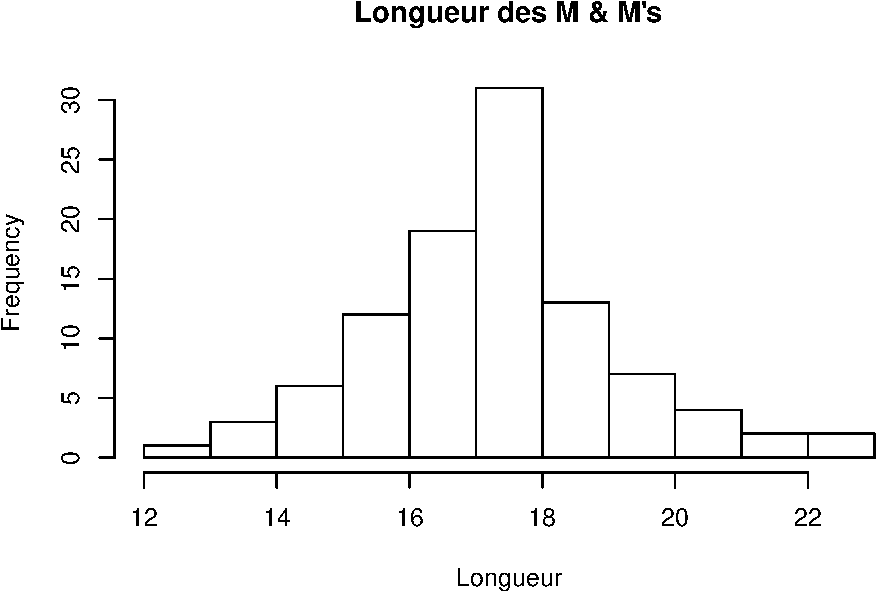
\includegraphics{TD1_files/figure-latex/unnamed-chunk-22-1.pdf}

\begin{Shaded}
\begin{Highlighting}[]
\KeywordTok{par}\NormalTok{(}\DataTypeTok{mfrow=}\KeywordTok{c}\NormalTok{(}\DecValTok{1}\NormalTok{,}\DecValTok{2}\NormalTok{))}
\KeywordTok{boxplot}\NormalTok{(}\DataTypeTok{data =}\NormalTok{ data2,}\StringTok{`}\DataTypeTok{Longueur maximale (mm)}\StringTok{`}\OperatorTok{~}\StringTok{ }\NormalTok{Couleur , }
        \DataTypeTok{main =} \StringTok{"Longueur des M & M's par couleur"}\NormalTok{,}
        \DataTypeTok{xlab=} \StringTok{"Couleur"}\NormalTok{, }\DataTypeTok{ylab=} \StringTok{"Taille"}\NormalTok{)}
\KeywordTok{boxplot}\NormalTok{(}\DataTypeTok{data =}\NormalTok{ data2,}\StringTok{`}\DataTypeTok{Poids (g)}\StringTok{`}\OperatorTok{~}\StringTok{ }\NormalTok{Couleur , }
        \DataTypeTok{main =} \StringTok{"Poid des M & M's par couleur"}\NormalTok{, }
        \DataTypeTok{xlab=} \StringTok{"Couleur"}\NormalTok{, }\DataTypeTok{ylab=} \StringTok{"Poid"}\NormalTok{)}
\end{Highlighting}
\end{Shaded}

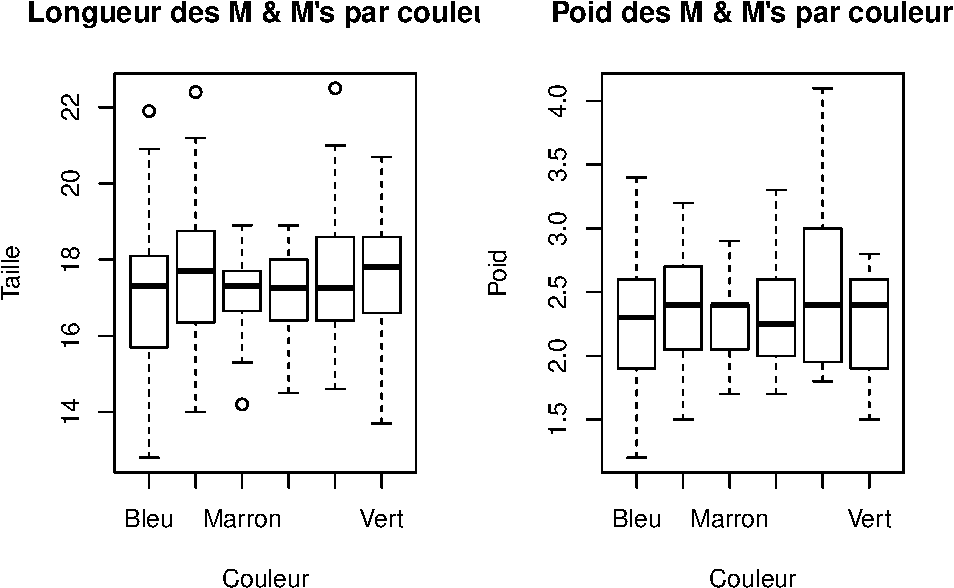
\includegraphics{TD1_files/figure-latex/unnamed-chunk-23-1.pdf}


\end{document}
